% !TEX TS-program = pdflatexmk
% !BIB TS-program = bibtex

\documentclass[12pt, a4paper, oneside]{book}
\usepackage{import}
\subimport{../}{preamble}
\standalonetrue
\onehalfspacing
\begin{document}

\begin{singlespace}
\color{white}\chapter{Microscope Design for Simultaneous Measurements on Plasmonic Tips}
\end{singlespace}

\AddToShipoutPictureBG*{ \AtPageUpperLeft{
\put(0,-250) {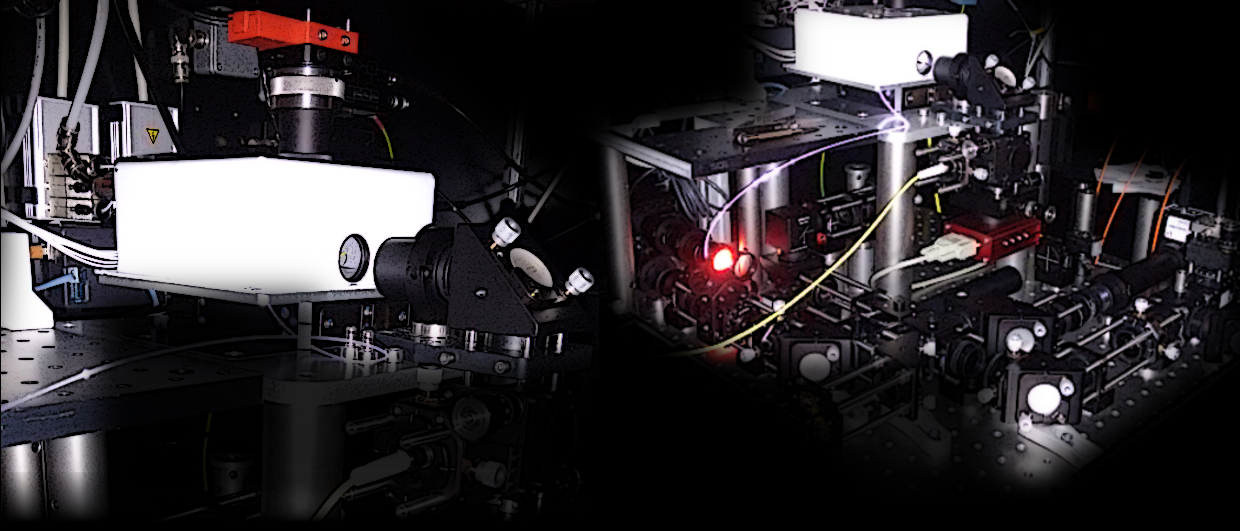
\includegraphics[width=\paperwidth]{../chapter_covers/test_rig_design_cover.png}}
\put(515,-5) {\begin{minipage}[t]{0.15\textwidth}\flushright\singlespace\fontsize{9pt}{1em}\selectfont\color{white} Images of the custom-built microscope platform.\end{minipage}}
}}

\Gls{afm} tip experiments are performed in a custom-built microscope for optical spectroscopy with simultaneous force and electronic measurements. The microscope is fully automated%
\footnote{A custom Python application used to control the microscope and all experiments}
and capable of running a variety of experiments, primarily to study the optical response of tips. Its primary function is to take the tips of two opposing AFM probes, align them into a tip-to-tip dimer geometry and demonstrate nanometric spatial control. Using such a setup, the plasmonic behaviour of both individual and coupled tip systems can be investigated. In this chapter the principles behind the operation and design considerations of the microscope system are discussed in depth, with sections split between the mechanical and optical design of the microscope followed by integration of the electronics and AFM module for force measurement.

\subimport{./}{mechanical_design}
\subimport{./}{optical_design}
\subimport{./}{electronics_design}
\subimport{./}{afm_design}
\subimport{./}{tip_alignment}

\section{Conclusions}

A custom-built ultra-stable microscope platform, utilising supercontinuum dark-field spectroscopy, low-noise electronics and AFM, is built to accommodate spectral studies of both individual tips and tip dimers. The platform is stable to both temperature and vibration and is able to take two tips and align them into a dimer configuration using a modified form of scanning capacitance microscopy. Performance characterisation shows spectral validity between 500--\SI{1100}{nm}, more broadband than standard optical microscopes, with confocal localisation enabling the study of more complex structures than point scatterers. The addition of \si{fA} level current and AFM force measurements results in a system capable of characterising a sub-nm plasmonic dimer system in far more detail than ever before possible.

\ifstandalone
\begin{singlespace}
\printbibliography[notcategory=fullcited]
\end{singlespace}
\fi

\end{document}